
\aufgabe{}{1}

An RT entity changes its value periodically according to 
\begin{displaymath} 
y(t) = A_{0}.\sin(2\pi ft) 
\end{displaymath} 
with amplitude $A_{0}$ and frequency f . What is the maximum permissible frequency $f_{max}$ for the entity value if the entity is sampled with a period of $T_{sample}$ = 1 msec, and the maximum change of value
between two sampling points should never exceed 0.1\% of the full range value?

\begin{tikzpicture}
\node (rect) at (0,0) [draw, text width=17 cm, minimum height=12cm]{};
\node[below right, text width=17 cm] at (rect.north west) {
    \lsg{
    Please sketch a model here
    }
   };
\end{tikzpicture}

\aufgabe{}{1}

Explain the difference between safety and reliability in hard real-time systems.

\aufgabe{}{2}

Explain the term “signal conditioning” in hard real-time systems.

\aufgabe{}{2}

Discuss the advantages and disadvantes of a distributed architecture vs. a centralized
architecture in terms of cost, reliability, and safety.


\aufgabe{}{2}

Explain the terms offset, drift, drift rate, precision, and accuracy in the context of real-time
clocks. Use a sketch if appropriate.

\aufgabe{}{4}

 Assume k clocks behave maliciously faulty. How many clocks N do you need at least to
achieve clock synchronisation?

\pagebreak
\headheight = 78pt

\aufgabe{}{10}

Explain the difference between the accuracy and precision of a clock.

\aufgabe{}{3}

 Explain the difference between state correction and rate correction for distributed clocks

\aufgabe{}{5}

Describe the structure of a node. Why is it important to distinguish between the i-state and
the h-state of a node in an embedded system?

\aufgabe{}{5}

 What is the difference between a parametric RT image and a phase-sensitive RT image?
How can we create parametric RT images?

\pagebreak


\aufgabe{}{5}

Calculate the action delay in a distributed system with the following parameters:
dmax=10msec, dmin=2msec,
and a) no global time available, granularity of local time is 20$\mu$sec
and b) global time with granularity of 30$\mu$ sec.

\aufgabe{}{5}

What are the problems with event observations?

\pagebreak

\aufgabe{}{5}

What are the basic techniques for error detection?

\aufgabe{}{5}

Given a bandwidth of 10 Mbit/sec, a channel length of 1000 m, and a message length of 100
bits, what is the limit of the protocol efficiency that can be achieved at the media access
level of a bus system?

\aufgabe{}{5}

Given are four tasks which access resources (A,B,C):
$\tau$ 1 (r 0 = 10, C = 4, Prio=4; [A;1]), where the task executes for two time units, and then requests
the resource A.
$\tau$ 2 (r 0 = 7, C = 4, Prio=3; [A;1][B;1]), where the task executes for one time unit, and then
requests the resource A, and thereafter B.
$\tau$ 3 (r 0 = 4, C = 4, Prio=2; [B;1][C;1]), where the task executes for one time unit, and then
requests the resource B, and thereafter C.
$\tau$ 4 (r 0 = 4, C = 4, Prio=1; [A;5[B;2]][C;1]), where the task executes for two time units, then
requests the resource A, holds it for one time unit, and then makes a nested request for resource
B, and then requests C.
Notation: r 0 is the release or request time, C is the execution time, Prio is the priority of the tasks
(higher number means higher priority). [A;5] means request to resource A for five time units.
[A;a[B;b]] means a nested critical sections, where the usage of A includes in turn the usage of B,
and time a includes time b.
This task set shall be scheduled with two different resource access protocols.
3.1 Construct the schedule for this task set using the priority inheritance protocol. Use the the
diagram furnished below. On the first four lines draw the schedule of each task as if there
were no other tasks. On the last line, draw the resulting schedule. Do not use a different
diagram template.

3.2  Construct the schedule for this task set using the priority ceiling protocol. On the first
four lines draw the schedule of each task as if there were no other tasks. On the last
line, draw the resulting schedule. Use the diagram provided below. Do not use your own
diagram templates


3.3 Take a look at another periodic task set with periods Ti and the following parameters:
Is it possible to create a schedule that meets all deadlines using the rate monotonic
algorithm (RMA)? Please explain.
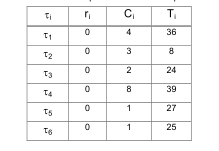
\includegraphics[width=0.7\textwidth]{master-exam-2009/2009_RMA}


3.4  Construct the schedule (mark using X) for the task set above and priority driven RMA into
the table below (two lines, second table is continuation of first table):

3.5 For the task set given in 3.3 consider the context switch time (the time it takes to
switch from execution of one task to another). This time shall take 0.8 time units, including
the start of the first job. Is it possible to create a valid schedule under these conditions?
Please explain.



